\section{Introduction}
\label{sec:intro}

%% Soft robots can do cool things because they are compliant, and need to be controlled
Soft robots incorporate non-rigid materials into their morphology to facilitate compliant interactions with the external world.
This compliance allows them to manipulate delicate objects, adapt to unstructured environments, and interact safely with coexisting humans 
% without the sophisticated sensing and control algorithms required by their rigid-bodied counterparts 
\cite{rus2015design}. \David{Yes, more references}
Since their utility is derived from their compliance, control methods that preserve and/or exploit this property are desirable. 

%% Models are necessary for control
Accurate models facilitate better control performance.
When an accurate model is available, predictive controllers can be built by using the model to calculate a feedforward term, then adding a feedback term to account for minor model uncertainty and disturbances.
% stabilize around that desired point/account for model uncertainty/error (i.e. make up the difference).
If a good model is unavailable, feedback must be more heavily relied upon.
This poses several problems for soft robots.
First, feedback requires sensing, but the morphology of soft robots precludes the use of many conventional sensors.
Suitable alternatives are currently in development \Dan{soft soft sensing papers}, but are not yet readily available.
Second, relying heavily on feedback to compensate for an inaccurate model has been illustrated to reduce the compliance of soft robotic systems \cite{della2017controlling}.
That is, excessive feedback negates the desirable compliance of a soft robot by replacing its natural dynamics with those of a slower, stiffer system.
Therefore, to control soft robots in a manner that reduces dependence on feedback and simultaneously preserves compliance, accurate models are required.
% Since feedback is reactionary rather than anticipatory it can be slow to track a set point and prone to unwanted oscillations.
% \David{Other arguments for models:  Controller development/tuning, design (even thought that is not an argument for a model that has been identified on hardware), observer (compute un-sensed states), load estimation, ...}

%% FIGURE: Overview Diagram
\begin{figure}[t]
    \centering
    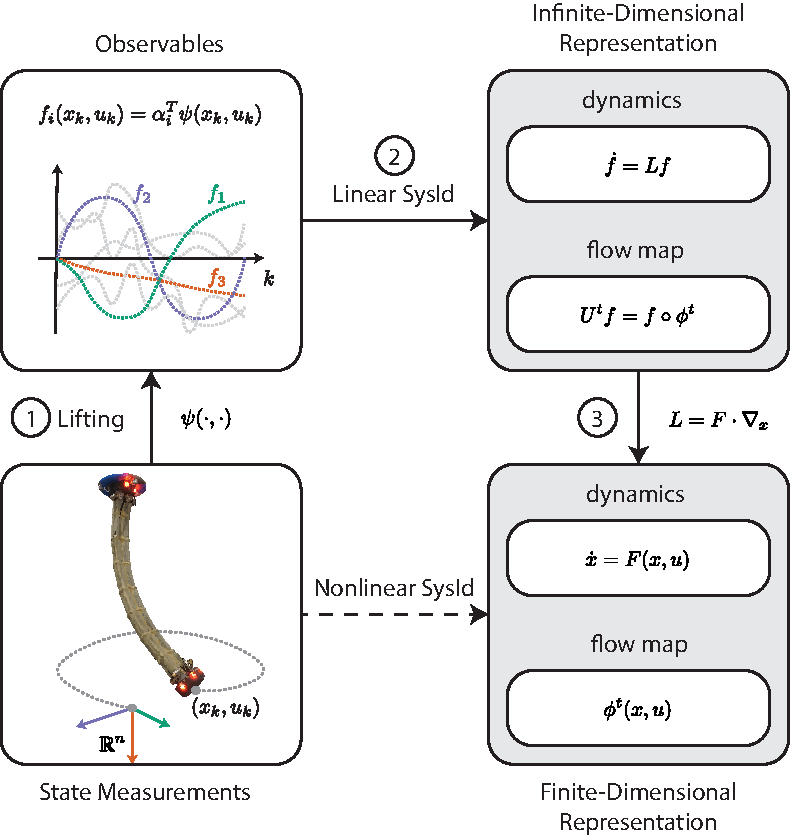
\includegraphics[width=\linewidth]{figures/overviewDiagram_wNumbers.pdf}
    \caption{ 
    \Ram{maybe mention that all of the notation is defined in Section 2}
    By providing an infinite-dimensional linear representation of a dynamical system, Koopman Operator Theory enables linear system identification of nonlinear systems. 
    This process proceeds in three steps.
    (1) Measured states of the system are lifted to the space of observables \Ram{what does that?}.
    (2) Least-squares regression is performed on the lifted data to obtain an approximation of the Koopman operator, $U^t$.
    (3) An approximation of the nonlinear vector field $\Fv$ is obtained via its one-to-one relationship with the Koopman operator.}
    \label{fig:overview}
\end{figure}


% Physics-based and data-driven models
Models for soft robots can be separated into two categories: physics-based models and data-driven models.
Physics-based models are constructed from observations of component material properties and first-principles, while data-driven models are constructed from observations of system behavior.
Physics-based models have the ability to make predictions about a system's behavior before the system is even constructed,
thus they can inform the design and construction of a soft robot intended for a particular task \cite{bishop2015design, bruder2018iros} \Dan{cite former FREE papers about design}.
%% Why physics-based models for soft robots are hard
However, the infinite degrees of freedom and hysteretic behavior of soft materials make it difficult to construct accurate physics-based models of soft robots without making simplifying assumptions such as constant curvature \cite{rus2015design}, quasi-static \cite{george2018control}, or simplified geometry \cite{bruder2017model, sedal2017constitutive, bishop2012parallel} \Ram{more references...}.
These models only describe behavior well in the subset of robot configurations where the assumptions hold, hence they are limited in applicability.
% This is bad for soft robots which are meant to be in contact with the world because they may often need to operate outside of regular specs
% For example, consider a linearization.
% By construction, the linear model describes system behavior well within some region of the equilibrium point
% \David{Talk to Audrey, she will have a good perspective about why it is hard to model soft robots.  I think other issues not mentioned here are computational cost, identification of material properties, influence of manufacturing tolerances,...}

%% Soft robots are particularly well suited for system identification
Data-driven models are more broadly applicable since they do not make structural assumptions about the system.
Data-driven models are constructed from observations of system behavior rather than from first-principles.
Hence, given sufficient data, they are capable of describing system behavior well over the entire range of observations.
% For the reasons stated above, it is typically not possible to construct globally accurate physics-based models of soft robots.
% In contrast, data-driven models are capable of describing system behavior well over the entire range of the observed data.
By virtue of their soft bodies, it is often possible to safely command arbitrary control inputs without risk of damaging a soft robot or nearby human operators.
Soft robots are therefore amenable to data collection over their entire operation range, making them particularly well suited for data-driven system identification techniques.

%% Nonlinear system identification is hard
To capture the characteristic nonlinear behaviors of most soft robots, identification of a nonlinear model is necessary.
Unfortunately, identifying a nonlinear model from data typically consists of solving a nonlinear non-convex optimization problem, for which global convergence is not guaranteed \cite{boyd2004convex}.
Furthermore, most nonlinear system identification methods require the manual initialization and tuning of training parameters, which have an obscure impact on the resulting model.
A neural network, for example, depends on the number of hidden layers, number of nodes per layer, activation function, and termination condition used during training, which must be selected through trial and error until acceptable results are achieved \cite{gillespie2018learning} \Dan{probably not the best to cite}.

%% Linear system identification is trivial
Linear model identification, on the other hand, does not suffer from the typical shortcomings of nonlinear identification 
since linear models can be identified via linear regression \cite{ljung1987system}.
However, linear models are poorly suited to capture the behavior of soft robots since their characteristic behavior is distinctly nonlinear \cite{rus2015design} \Dan{cite continuum paper}.
% However, linear models have a limited ability to capture the nonlinear behavior exhibited by most soft robots \cite{rus2015design} \Dan{cite continuum paper}


\Dan{deleted paragraph about neural network sysid paper}
%% Neural network has successfully been applied to soft robot
% Despite its challenges, nonlinear system identification of a soft robot has been performed in the past.
% In \cite{gillespie2018learning}, for instance, a Deep Neural Network (DNN) was used to model the behavior of a 1 DOF pneumatic soft robot arm.
% The resulting model predictive controller (MPC) with the neural network model acting as its predictor performed comparably to an MPC controller with a much more complicated physics-based model.
% While in this case the neural network model was effective, a weakness of neural network models in general is the extent to which the training process is heuristic in nature.
% A neural network model depends on the specific training parameters chosen (e.g. number of hidden layers, number of nodes per layer, activation function, termination condition), which must be selected through trial and error until acceptable results are achieved.

%% Koopman let's us do linear sysid (trivial) on a nonlinear system
In this work, we employ Koopman operator theory to generate nonlinear, data-driven models of soft robots via linear regression.
This approach, which is described in greater detail in Section \ref{sec:theory}, relies on the idea of lifting nonlinear dynamical systems to an infinite dimensional space, where those systems have a linear representation.
In this space, it is possible to describe the dynamic behavior of a system by a linear operator rather than a nonlinear vector field (see Fig. \ref{fig:overview}).
This linear operator, called the Koopman operator, is identified via linear regression, so it does not suffer from the convergence and tuning problems that are characteristic of neural networks other nonlinear system identification methods.


%% Contributions (Why is this contribution significant?: Could enable real-time sysid/control, MPC)
Our primary contribution is demonstrating, on a real system, a data-driven method for constructing globally valid nonlinear models that does not require the manual tuning of training parameters.
To do so, we apply the Koopman based system identification method described in \cite{mauroy2016linear} and \cite{mauroy2017koopman} to create a dynamic model of a soft robot arm and verify that it captures the system's true dynamic behavior better than the models generated by several other state-of-the-art nonlinear system identification methods including a neural network, a nonlinear auto-regressive moving average model with exogenous inputs (NARMAX), a nonlinear Hammerstein-Wiener, and a state space model.
To the author's knowledge, this technique has never before been used to identify the dynamic model of a real system, much less a soft robot.
We believe that this system identification method applied to soft robots will enable the rapid development of new and effective control strategies by making accurate nonlinear dynamic models easier to construct.


%% Outline of the rest of this paper
The rest of this paper is organized as follows:
In Section \ref{sec:theory} we formally introduce the Koopman operator and describe the system identification method. 
In Section \ref{sec:experiment} we describe the soft robot and experimental procedure used for collecting input-output data of the system.
In Section \ref{sec:results} we summarize the results of applying various nonlinear system identification techniques to the collected data and compare the performances of the models generated. 
Concluding remarks and perspectives are provided in Section \ref{sec:conclusion}.